\documentclass{article}
\usepackage{graphicx}
\usepackage{amsmath}
\usepackage{geometry}
\usepackage{tikz}
\usepackage{hyperref}
\usepackage{pgfplots}
\pgfplotsset{compat=1.17}
\usetikzlibrary{shapes.geometric, arrows, positioning, fit, calc}
\geometry{a4paper, margin=1in}

\title{MCUMotionNet: A Lightweight, Two-Stage Architecture for Real-Time Object Tracking on Memory-Constrained Microcontrollers}
\author{Sébastien Campion}
\date{\today}

\begin{document}

\maketitle

\begin{abstract}
The proliferation of Tiny Machine Learning (TinyML) has pushed the boundaries of what is possible on low-power, resource-constrained microcontrollers (MCUs).
However, complex tasks like real-time video analysis and object tracking remain a significant challenge due to strict memory and computational limits.
This paper introduces MCUMotionNet, a novel two-stage deep learning architecture designed for real-time target tracking on MCUs with as little as 512KB of RAM.
The architecture first employs a highly efficient object detector based on a truncated MobileNetV2 backbone and a Faster Objects, More Objects (FOMO) head to locate target centroids.
Subsequently, a recurrent neural network (RNN) head processes temporal sequences of features to predict the necessary camera motion to keep a target in frame.
We describe the model's application in tracking a handball player to automatically control a panoramic camera turret.
We detail the experimental setup, including various configurations of the RNN head, which were trained on the Leonardo EuroHPC supercomputer to evaluate the trade-off between model complexity and tracking performance.
The results demonstrate the viability of our approach for deploying sophisticated, real-time video-based tracking systems on edge devices.
\end{abstract}

\section{Introduction}
The Internet of Things (IoT) has led to an explosion of smart devices, creating a demand for processing data directly at the source, a paradigm known as edge computing.[1, 2] This shift is driven by the inherent limitations of cloud-based AI, such as unacceptable latency for time-sensitive applications, high bandwidth and energy costs for continuous data streaming, and significant data privacy concerns.[1, 3] Tiny Machine Learning (TinyML) represents the cutting edge of this trend, focusing on the deployment of machine learning models on microcontrollers (MCUs) characterized by their low cost, low power consumption (often sub-milliwatt), and minimal resources—typically with only kilobytes of RAM and flash memory.[4, 5, 6]

While TinyML has seen success in applications like keyword spotting and simple anomaly detection, tasks involving real-time video streams, such as object tracking, have remained largely out of reach.[4] Traditional deep learning models for object detection and tracking are notoriously resource-intensive, often requiring billions of parameters and powerful GPUs.[6] This paper addresses the challenge of implementing a real-time, video-based tracking system on a severely constrained MCU, specifically targeting a device with under 512KB of available RAM.

Our use case is the automated control of a camera turret designed to follow a player during a handball match. This application sits at the intersection of TinyML and automated sports analysis, a domain currently dominated by expensive, high-power edge devices or cloud-based systems.[7, 8, 9] Our approach requires not only detecting the player in each frame but also understanding their motion over time to predict the correct camera movement. To solve this, we propose MCUMotionNet, a specialized neural network architecture that combines efficient object detection with temporal sequence processing.\footnote{The source code for this project is available at: \url{https://github.com/scampion/MCUMotionNet}} The key contributions of this work are:
\begin{itemize}
    \item A novel two-stage architecture combining a MobileNetV2-FOMO detector with a lightweight RNN head for motion prediction, designed explicitly for MCU constraints.
    \item A demonstration of a complete system for real-time object tracking and camera control on a memory-constrained MCU.
    \item An analysis of different RNN head configurations to explore the performance-versus-complexity trade-off, with models trained on the Leonardo EuroHPC infrastructure.
\end{itemize}

\section{Related Work}
Our work builds upon several key advancements in efficient deep learning, temporal modeling, and automated sports analysis.

\subsection{Efficient On-Device Object Detection}
\textbf{MobileNetV2:} The MobileNet family of architectures is a cornerstone of efficient deep learning for mobile and edge devices.[10] MobileNetV2, in particular, introduced the inverted residual with linear bottleneck, a memory-efficient block that uses lightweight depthwise separable convolutions to filter features within an expanded, higher-dimensional space before projecting them back to a low-dimensional representation.[11, 12, 13] This structure provides a powerful yet lightweight feature extractor, and we use a truncated version as the backbone of our object detector.

\textbf{FOMO (Faster Objects, More Objects):} For object detection on the extreme edge, traditional models that rely on bounding box regression are often too slow and complex.[14] The FOMO paradigm, introduced by Edge Impulse, reframes object detection as a classification problem on a grid of the image.[15, 16, 17, 18] Instead of predicting bounding box coordinates, it identifies the centroids of objects by producing a heatmap. This simplification dramatically reduces computational load and model size, making it ideal for MCU-based applications, capable of achieving over 30 FPS on Cortex-M7 cores in under 200KB of RAM.[18, 19] However, this efficiency comes with limitations, such as difficulty in detecting objects of varying sizes or those with overlapping centroids, which motivates our two-stage design.[20, 21]

\subsection{Temporal Motion Modeling}
The MCUMotionNet architecture follows the well-established "tracking-by-detection" paradigm, where objects are first detected in individual frames and then associated across time to form trajectories.[22, 23] While effective, running a detector on every frame is often too costly for embedded devices.[23] Our two-stage system embodies this principle by separating spatial detection (Stage 1) from temporal prediction (Stage 2).

To model temporal dynamics, Recurrent Neural Networks (RNNs) are a natural choice due to their ability to maintain an internal state, or "memory," of past events.[22, 24] Architectures like Long Short-Term Memory (LSTM) and Gated Recurrent Unit (GRU) use gating mechanisms to overcome the vanishing gradient problem in simple RNNs, allowing them to learn long-term dependencies in sequential data.[24] These models have been successfully applied to predict human motion and object trajectories in video streams.[25, 26, 27, 28] Our work adapts these principles by using a ConvLSTM2D layer, which preserves the spatial structure of the feature maps while processing them temporally, to predict camera motion from a sequence of detected object features.

\subsection{Automated Sports Broadcasting}
The application of computer vision to automate sports broadcasting and analysis is a rapidly growing field.[29, 30] Commercial systems from companies like Pixellot, Veo, and XbotGo use AI to automatically track the action, produce broadcast-style video feeds, and provide analytics without a human operator.[31, 7, 32, 8, 9] These systems typically rely on powerful edge computers (e.g., NVIDIA Jetson) or cloud processing and are targeted at professional leagues and clubs with significant budgets.[33, 34] MCUMotionNet addresses a critical gap in this market by demonstrating the feasibility of deploying a useful player tracking and camera control system on inexpensive, low-power microcontrollers, thereby democratizing access to automated sports video technology.

\section{MCUMotionNet Architecture}
MCUMotionNet is a two-stage, multi-head model designed to process a sequence of images and produce two distinct outputs: an object detection heatmap for the current frame and a motion prediction value based on the sequence. The architecture is detailed in the \texttt{create\_fomo\_td\_with\_rnn\_combined\_model} function in our codebase and visualized in Figure \ref{fig:architecture}.
\begin{figure}[h!]
\centering
\resizebox{\textwidth}{!}{%
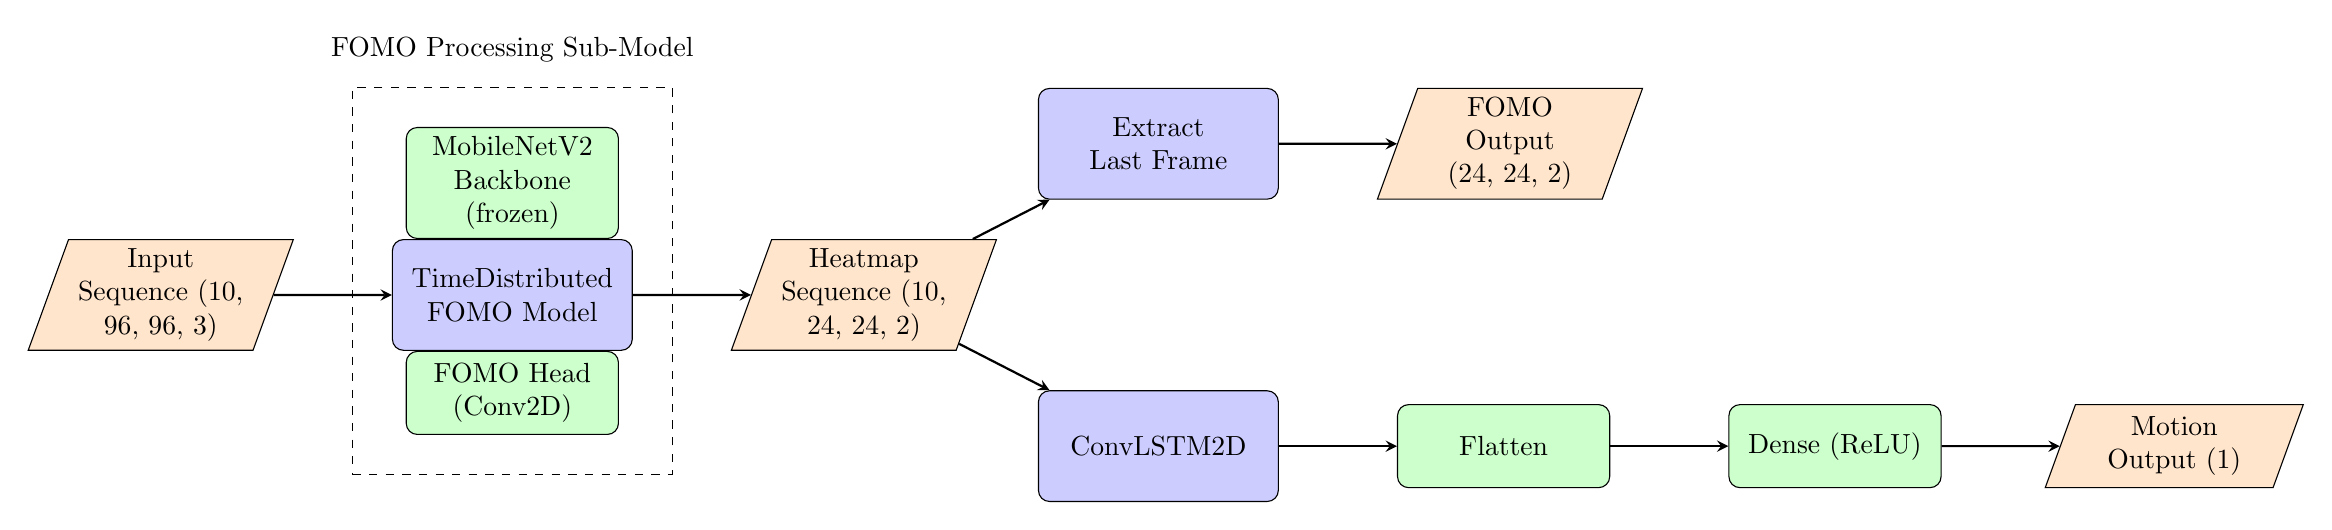
\begin{tikzpicture}[
    node distance=0.5cm and 1.5cm,
    block/.style={rectangle, draw, fill=blue!20, text width=8em, text centered, rounded corners, minimum height=4em},
    smallblock/.style={rectangle, draw, fill=green!20, text width=7em, text centered, rounded corners, minimum height=3em},
    arrow/.style={thick,->,>=stealth},
    line/.style={thick,-},
    io/.style={trapezium, trapezium left angle=70, trapezium right angle=110, draw, fill=orange!20, text width=6em, text centered, minimum height=3em},
    container/.style={rectangle, draw, dashed, inner sep=0.5cm}
]

% Nodes

\node[io] (input) {Input Sequence (10, 96, 96, 3)};
% TimeDistributed FOMO Model

\node[block, right=of input] (td_fomo) {TimeDistributed FOMO Model};

\node[smallblock, above=of td_fomo, yshift=-0.5cm] (fomo_backbone) {MobileNetV2 Backbone (frozen)};
\node[smallblock, below=of td_fomo, yshift=0.5cm] (fomo_head) {FOMO Head (Conv2D)};

% Dashed box for the sub-model

\node[container, fit=(fomo_backbone) (td_fomo) (fomo_head), label={[yshift=0.2cm]above:FOMO Processing Sub-Model}] (fomo_container) {};
\draw[arrow] (input) -- (td_fomo);

% Sequence Output

\node[io, right=of td_fomo] (seq_output) {Heatmap Sequence (10, 24, 24, 2)};
\draw[arrow] (td_fomo) -- (seq_output);
% Branch 1: FOMO Output

\node[block, above right=of seq_output] (lambda) {Extract Last Frame};
\node[io, right=of lambda] (fomo_output) {FOMO Output (24, 24, 2)};
\draw[arrow] (seq_output) -- (lambda);
\draw[arrow] (lambda) -- (fomo_output);
% Branch 2: Motion Prediction

\node[block, below right=of seq_output] (convlstm) {ConvLSTM2D};

\node[smallblock, right=of convlstm] (flatten) {Flatten};
\node[smallblock, right=of flatten] (dense) {Dense (ReLU)};

\node[io, right=of dense] (motion_output) {Motion Output (1)};

\draw[arrow] (seq_output) -- (convlstm);
\draw[arrow] (convlstm) -- (flatten);
\draw[arrow] (flatten) -- (dense);
\draw[arrow] (dense) -- (motion_output);

\end{tikzpicture}
}
\caption{The MCUMotionNet architecture.
A TimeDistributed FOMO model processes an input sequence of 10 frames.
The output splits into two heads: one extracts the final FOMO heatmap for object detection, and the other uses a ConvLSTM2D layer to process the full sequence for motion prediction.}
\label{fig:architecture}
\end{figure}

\subsection{Stage 1: FOMO-based Person Detector}
The first stage is a person detector based on the FOMO architecture, designed to be applied to each frame of an input video sequence.
\begin{itemize}
    \item \textbf{Backbone:} We use a MobileNetV2 model with a width multiplier (\texttt{alpha}) of 0.35 as the feature extractor.[11, 12, 13]
To keep the model small and increase the output resolution of the feature map, we truncate the backbone at the \texttt{block\_3\_expand\_relu} layer.
This results in a feature map with a spatial reduction factor of 4 (e.g., a 96x96 image produces a 24x24 feature map).
\item \textbf{Head:} A simple convolutional head is attached to the backbone output.
It consists of a 1x1 convolution to process the features, followed by another 1x1 convolution that produces a final heatmap.
This heatmap has dimensions corresponding to the feature map grid (e.g., 24x24), with a channel depth equal to the number of classes plus one for the background.
Each cell in the grid represents a classification of whether an object's centroid is present at that location.[15, 16, 18]
\end{itemize}
This entire FOMO model is encapsulated in a \texttt{TimeDistributed} layer, allowing it to be applied independently to each of the 10 frames in the input sequence.
\subsection{Stage 2: RNN Motion Prediction Head}
The second stage is an RNN that analyzes the temporal information contained within the sequence of feature maps generated by the FOMO stage.
\begin{itemize}
    \item \textbf{Input:} The RNN head takes the output of the \texttt{TimeDistributed} FOMO model as its input.
This is a sequence of heatmaps of shape (10, 24, 24, 2), where 10 is the sequence length, (24, 24) is the grid size, and 2 is for the 'person' and 'background' classes.
\item \textbf{Recurrent Layer:} A \texttt{ConvLSTM2D} layer processes this sequence. \texttt{ConvLSTM2D} is well-suited for spatiotemporal data as it maintains the spatial structure (2D grid) of the input while processing it sequentially.[24]
It processes the entire sequence and returns a single output feature map.
\item \textbf{Output Layers:} The feature map from the \texttt{ConvLSTM2D} layer is flattened and passed through a \texttt{Dense} layer with a ReLU activation, followed by a final \texttt{Dense} output layer with a \texttt{tanh} activation.
This final layer outputs a single continuous value between -1 and 1, representing the predicted camera motion (pan left/right).
\end{itemize}

\subsection{Combined Model and Training Strategy}
The final model has a single input for an image sequence and two outputs:
\begin{enumerate}
    \item \textbf{FOMO Output:} The object detection heatmap from the very last frame in the sequence.
\item \textbf{Motion Output:} The motion prediction value from the RNN head.
\end{enumerate}
The training is performed in two stages.
First, the FOMO person detector is trained separately on a dataset of annotated single images.
Then, in the second stage, its weights are loaded into the combined model and frozen.
Only the RNN head (ConvLSTM and Dense layers) is trained on sequences of video frames with corresponding motion labels.
This strategy allows the model to first learn a robust visual representation and then learn the temporal dynamics for motion prediction.

\section{Experimental Setup}
All Stage 2 training experiments were conducted on the Leonardo EuroHPC supercomputer.
\subsection{Dataset and Preprocessing}
The training data was created by extracting short video clips of handball matches from the sport.video platform\footnote{\url{https://sport.video}}.
These clips, typically lasting a few seconds, capture dynamic player movements suitable for training a motion tracking model.
An example of a source video can be found at \url{https://sport.video/slovnaft-handball-extraliga/play-off-207000002/hkm-sala-vs-msk-povazska-bystrica-207000042/v310a08f9c-575b-4c5a-bf38-d3ddfcb575d9}.
To generate the ground truth for camera motion, we developed a data preparation pipeline using the script found at \texttt{preparation/compute\_camera\_movement.py}.
This script processes each video clip to estimate the global camera movement between consecutive frames.
It employs the Lucas-Kanade optical flow algorithm (\texttt{cv2.calcOpticalFlowPyrLK}) on a set of tracked feature points to calculate the average horizontal (\texttt{Move\_X}) and vertical (\texttt{Move\_Y}) displacement.
This displacement vector represents the motion required to stabilize the frame, and thus serves as the supervision signal for training the RNN head to predict camera adjustments.
The \texttt{Move\_X} value is clipped and normalized to the range [-1, 1] to serve as the final ground truth label.
The complete dataset, containing the video sequences and their corresponding motion annotation files, is publicly available on Hugging Face\footnote{\url{https://huggingface.co/datasets/scampion/handball_video_sequences}}.
Input frames are resized to 96x96 pixels and normalized. The model takes sequences of 10 consecutive frames as input.

\subsection{Training Process}
The RNN head of the combined model is trained using the Adam optimizer with an initial learning rate of 0.0005.
The loss function for the motion prediction output is Mean Squared Error (MSE), as it is a regression task.
We monitor the validation loss and use callbacks for early stopping, learning rate reduction on plateau, and model checkpointing.

\subsection{Performance Metrics}
Evaluating models for TinyML is an exercise in multi-objective optimization, balancing task performance against strict hardware constraints.[35, 36] We evaluate our models based on the following key metrics:
\begin{itemize}
    \item \textbf{Model Accuracy:} For the motion prediction task, we use Mean Absolute Error (MAE) on the validation set to measure the accuracy of the predicted camera movement.
    \item \textbf{Model Complexity:} We consider the number of parameters and multiply-accumulate operations (MACs) as proxies for on-device performance.
    \item \textbf{Resource Usage:} The primary constraints are the final model size (for Flash memory) and the peak memory usage during inference (for RAM). The target is a total RAM footprint under 512KB.[37, 38, 39]
    \item \textbf{Latency:} The ultimate goal is to achieve a high enough frame rate (FPS) for real-time tracking on the target MCU. This is directly related to the model's complexity and its implementation on the hardware.[23, 40]
\end{itemize}

\subsection{Model Variations}
To find the best balance between performance and model size, we defined a series of experiments, each with a different configuration for the RNN head.
The complexity of the \texttt{ConvLSTM2D} layer (number of filters) and the subsequent \texttt{Dense} layer (number of units) were varied.

\section{Results and Discussion}
The training logs for the experiments listed in Table \ref{tab:experiments} were generated on the Leonardo supercomputer and are stored in the \texttt{logs\_leo/} directory.
A full quantitative analysis requires parsing these TensorBoard event files to extract the final validation metrics (e.g., Mean Absolute Error) and calculating the precise final model size for each configuration after quantization.
\begin{figure}[h!]
\centering
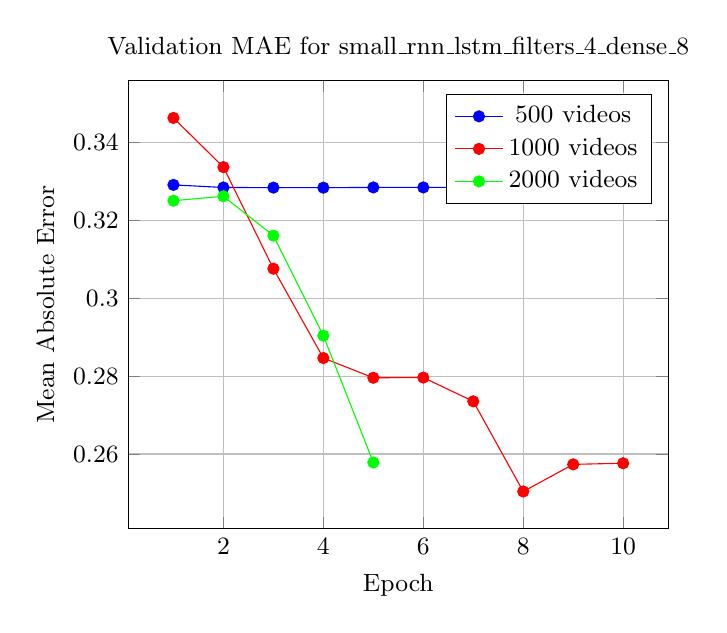
\begin{tikzpicture}
\begin{axis}[
    title={Validation MAE for small\_rnn\_lstm\_filters\_4\_dense\_8},
    xlabel={Epoch},
    ylabel={Mean Absolute Error},
    grid=major,
    legend pos=north east,
    title style={font=\small},
    tick label style={font=\small},
    label style={font=\small},
    legend style={font=\small}
]
\addplot[
    color=blue,
    mark=*,
]
coordinates {
    (1, 0.329065)
    (2, 0.328398)
    (3, 0.328363)
    (4, 0.328348)
    (5, 0.328414)
    (6, 0.328414)
    (7, 0.328401)
    (8, 0.328349)
   
 (9, 0.328359)
    (10, 0.328346)
};
\addplot[
    color=red,
    mark=*,
]
coordinates {
    (1, 0.346247)
    (2, 0.333620)
    (3, 0.307557)
    (4, 0.284629)
    (5, 0.279569)
    (6, 0.279619)
    (7, 0.273523)
    (8, 0.250376)
    (9, 0.257347)
    (10, 0.257633)
};
\addplot[
    color=green,
    mark=*,
]
coordinates {
    (1, 0.324999)
    (2, 0.326147)
    (3, 0.316049)
    (4, 0.290376)
    (5, 0.257830)
};
\legend{500 videos, 1000 videos, 2000 videos}
\end{axis}
\end{tikzpicture}
\caption{Validation Mean Absolute Error over training steps for the \texttt{small\_rnn} configuration with 500, 1000, and 2000 training videos.}
\label{fig:validation_mae_small_rnn}
\end{figure}

However, the experimental design allows us to discuss the expected trade-offs.
The "extra\_small\_rnn" configuration is expected to produce the smallest and fastest model, making it the most likely candidate to fit within the strict 512KB RAM limit of the target MCU.
As we move towards the "extra\_large\_rnn" configuration, the model's capacity to learn complex temporal patterns increases, which should lead to lower validation error and more accurate tracking.
This increased complexity, however, comes at the cost of a larger model size and higher computational requirements, potentially exceeding the hardware's capabilities.[35, 41]

In contrast to the successful training of the smaller models, the \texttt{medium\_rnn} configuration (with 8 ConvLSTM filters and a 16-unit Dense layer) failed to converge, as shown in Figure \ref{fig:validation_mae_medium_rnn}.
The validation MAE increased over the first few epochs, indicating that the model was not learning the desired task.
This behavior is a strong indicator of overfitting or that the network architecture was too complex for the amount of training data provided.
The increased number of parameters may have allowed the model to memorize noise in the training set rather than generalizing, leading to poor performance on the validation set.
This highlights the critical importance of model selection in resource-constrained environments, where simpler models are often more robust.
The goal of this experimental sweep is to identify the "sweet spot": the simplest model configuration that provides "good enough" tracking performance for the handball use case while comfortably meeting the hardware constraints.
\begin{figure}[h!]
\centering
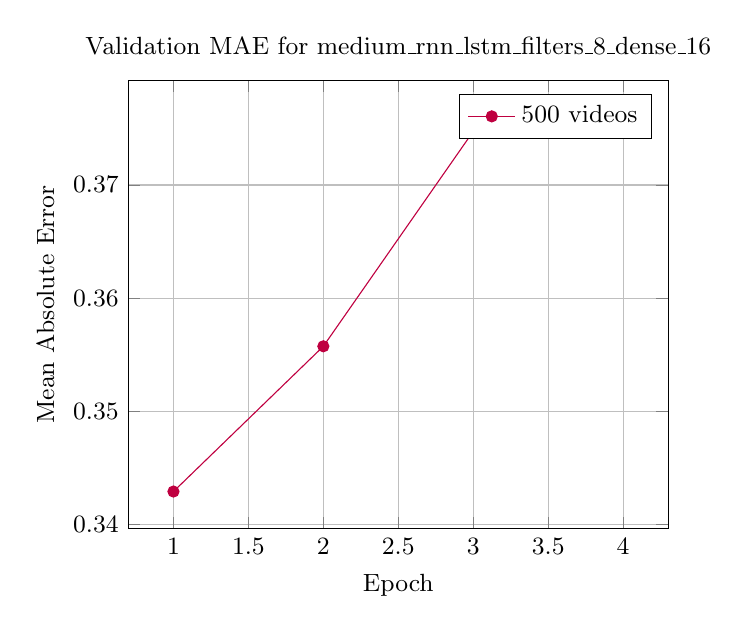
\begin{tikzpicture}
\begin{axis}[
    title={Validation MAE for medium\_rnn\_lstm\_filters\_8\_dense\_16},
    xlabel={Epoch},
    ylabel={Mean Absolute Error},
    grid=major,
    legend pos=north east,
    title style={font=\small},
    tick label style={font=\small},
    label style={font=\small},
    legend style={font=\small}
]
\addplot[
    color=purple,
    mark=*,
]
coordinates {
    (1, 0.342921)
    (2, 0.355750)
    (3, 0.374735)
    (4, 0.375921)
};
\legend{500 videos}
\end{axis}
\end{tikzpicture}
\caption{Failed training run for the \texttt{medium\_rnn} configuration, showing increasing validation MAE.}
\label{fig:validation_mae_medium_rnn}
\end{figure}

\section{Conclusion}

This paper presented MCUMotionNet, a lightweight, two-stage neural network architecture for real-time object tracking on resource-constrained microcontrollers.
By combining a highly efficient FOMO-based object detector with a temporal RNN, our model can perform both object localization and motion prediction, making it suitable for controlling an automated camera turret.
We have detailed the architecture, which is grounded in established principles of efficient deep learning and temporal sequence modeling, and situated our work within the application context of automated sports analysis. We also outlined the experimental framework used to evaluate different model complexities against key TinyML performance metrics.
The work demonstrates a clear path toward enabling sophisticated, real-time video analysis on the smallest of edge devices, potentially democratizing technology previously limited to high-cost, professional systems.
Future work will involve completing the quantitative analysis of the experimental results, quantizing the best-performing model, and deploying it on the target ESP32-S3 hardware to measure real-world performance, including latency and power consumption.

\begin{thebibliography}{99}

\bibitem{mobilenetv2}
Sandler, M., Howard, A., Zhu, M., Zhmoginov, A., \& Chen, L. C. (2018).
\textit{MobileNetV2: Inverted Residuals and Linear Bottlenecks}.
In Proceedings of the IEEE Conference on Computer Vision and Pattern Recognition (CVPR).

\bibitem{fomo_edgeimpulse}
Edge Impulse. (n.d.).
\textit{FOMO: Faster Objects, More Objects}.
Edge Impulse Documentation.

\bibitem{tinyml_survey_1}
Zhang, Y., et al. (2024).
\textit{From TinyML to TinyDL: A Comprehensive Survey of Deep Learning on Microcontrollers}.
arXiv preprint arXiv:2506.18927.

\bibitem{tinyml_survey_2}
Capogrosso, L., Ziviani, D., et al. (2024).
\textit{A Machine Learning-Oriented Survey on Tiny Machine Learning}.
IEEE Access.

\bibitem{fedosov2024key}
Fedosov, A., et al. (2024).
\textit{Key Considerations for Real-Time Object Recognition on Edge Computing Devices}.
Applied Sciences.

\bibitem{lin2020mcunet}
Lin, J., et al. (2020).
\textit{MCUNet: Tiny Deep Learning on IoT Devices}.
Advances in Neural Information Processing Systems.

\bibitem{boyle2024dsort}
Boyle, L., Moosmann, J., Baumann, N., Heo, S., \& Magno, M. (2024).
\textit{DSORT-MCU: Detecting Small Objects in Real-Time on Microcontroller Units}.
IEEE Sensors Journal.

\bibitem{tracking_by_detection_survey}
Yoon, S., et al. (2021).
\textit{Multiple Object Tracking in Deep Learning Approaches: A Survey}.
Sensors.

\bibitem{milan2017online}
Milan, A., et al. (2017).
\textit{Online Multi-Target Tracking Using Recurrent Neural Networks}.
In AAAI Conference on Artificial Intelligence.

\bibitem{martinez2017human}
Martinez, J., et al. (2017).
\textit{On Human Motion Prediction Using Recurrent Neural Networks}.
In Proceedings of the IEEE Conference on Computer Vision and Pattern Recognition.

\bibitem{carr2016autonomous}
Carr, P., et al. (2016).
\textit{Autonomous Camera Systems: A Survey}.
AI Magazine.

\bibitem{pixellot_handball}
Pixellot. (n.d.).
\textit{Handball AI Tracking Camera \& Video Analysis Software}.
Retrieved from Pixellot official website.

\bibitem{veo_camera}
Veo. (n.d.).
\textit{Veo Sports Video Camera: Smart AI Analysis for Teams}.
Retrieved from Veo official website.

\bibitem{xbotgo_camera}
XbotGo. (n.d.).
\textit{AI Powered \& Auto Tracking Camera System for Sports}.
Retrieved from XbotGo official website.

\bibitem{banbury2021mlperf}
Banbury, C., Reddi, V. J., et al. (2021).
\textit{MLPerf Tiny Benchmark}.
arXiv preprint arXiv:2106.07690.

\bibitem{machado2022benchmarking}
Machado, P., et al. (2022).
\textit{Benchmarking Object Detection Deep Learning Models in Embedded Devices}.
Sensors.

\end{thebibliography}

\end{document}
